% LaTeX Article Template - customizing header and footer
\documentclass{article}

\newtheorem{thm}{Theorem}

% Set left margin - The default is 1 inch, so the following 
% command sets a 1.25-inch left margin.
\setlength{\oddsidemargin}{0.25in}

% Set width of the text - What is left will be the right margin.
% In this case, right margin is 8.5in - 1.25in - 6in = 1.25in.
\setlength{\textwidth}{6in}

% Set top margin - The default is 1 inch, so the following 
% command sets a 0.75-inch top margin.
\setlength{\topmargin}{-0.25in}

% Set height of the header
\setlength{\headheight}{0.3in}

% Set vertical distance between the header and the text
\setlength{\headsep}{0.2in}

% Set height of the text
\setlength{\textheight}{9in}

% Set vertical distance between the text and the
% bottom of footer
\setlength{\footskip}{0.1in}

% Set the beginning of a LaTeX document
\usepackage{multirow}

\usepackage{tikz}

\usepackage{fullpage}
\usepackage{graphicx}
\usepackage{amsthm}
\usepackage{url}
\usepackage{amssymb}
\usepackage{amssymb}
\usepackage{algpseudocode}
\graphicspath{%
    {converted_graphics/}% inserted by PCTeX
    {/}% inserted by PCTeX
}
%%%%%%%%%%%%%%%%%%%%%%%%%%%%%




\begin{document}\title{Homework $2$\\ Computer Science \\ B351 Spring 2017\\ Prof. M.M. Dalkilic}         % Enter your title between curly braces
\author{James Gregory}        % Enter your name between curly braces
\date{\today}          % Enter your date or \today between curly braces
\maketitle


% Redefine "plain" pagestyle
\makeatother     % `@' is restored as a "non-letter" character




% Set to use the "plain" pagestyle
\pagestyle{plain}
All the work herein is mine.
\section*{Introduction}
The aim of this homework is to get you acquianted with problem solving and the steps  (Real World $\rightarrow$ Concept $\rightarrow$ Logic  $\rightarrow$ Implementation).  You will turn-in four files\begin{itemize} \item A *pdf with the written answers called \texttt{h2.pdf} \item A Python script called \texttt{rv1.py} \item  A Python script called  \texttt{rv2.py} \item A Python script called \texttt{rpsg.py} for rock-paper-scissors.\end{itemize}.  If you've attempted extra credit, add the comment \#ExtraCredit to the programs and ExtraCredit to the homework near the top so it's visible and obvious.  I am providing this \LaTeX{} document for you to freely use as well. Please enjoy this homework and ask yourself what interests you and then how can you add that interest to it!  Finally, each homework question is worth 100 points.
\newpage
\section*{Homework Questions}
\begin{enumerate}
\item Problem 3.10 (p. 115) in the text.
\begin{quote}
\textbf{State:} a configuration a problem can exist in. \newline
\textbf{State Space:} all of the possible configurations that can exist for a given problem. \newline
\textbf{Search Tree:} a collection of Search Nodes which begins with a root node, and ends with leaf nodes (nodes with all null children). \newline
\textbf{Search Node:} an object containing data and a collection of child nodes. Some, or all, children can be null. \newline 
\textbf{Goal:} a State within a State Space that is closest to a user-defined "ideal." \newline
\textbf{Action:} choosing which child Node to move to from a parent Node. \newline
\textbf{Transition Model:} a collection of resulting States from taking each possible Action from a given State. \newline
\textbf{Branching Factor:} the number of children each State in a State Space has.
\end{quote}
\item Problem 3.18 (p. 117) in the text.
\begin{quote}
An iterative deepening search will perform much worse than a depth-first search in a state space with a branching factor greater than 1, where all goal nodes have equal, large heights and a goal node exists far to the left.
\end{quote}
\item The text (page 95) describes consistency as:
\begin{eqnarray*}
h(n) &\leq c(n,a,n') + h(n')
\end{eqnarray*}
for state $n$, its successor $n'$ and action $a$.  For $G = (\{A,B,C\},\{(A,B), (A,C), (B,C)\})$, $Cost = \{((A,B),2), ((A,C),5), ((B,C), 1)\}$, and $h(A) = 1, h(B) = 4, h(C) = 3$. Is this consistent?
\begin{quote}
If $G$ is a directed graph, where each $u \in E(u,v)$ is the parent, this heuristic is consistent:
\newline 
$h(A) \leq c(A, B) + h(B) \equiv 1 \leq 2 + 4$\newline
$h(A) \leq c(A, C) + h(C) \equiv 1 \leq 5 + 3$\newline
$h(B) \leq c(B, C) + h(C) \equiv 4 \leq 1 + 3$
\end{quote}
\begin{quote}
If $G$ is an undirected graph, this heuristic is not consistent because: \newline
$h(B) > c(A, B) + h(A) \equiv 4 > 2 + 1$
\end{quote}

\item Assume you're programming a robot named \textsf{R} to navigate a 2D surface.  The robot can only move forward a single step to an adjacent square (not diagonally), but can also rotate $\pm$ 90 degrees.  \textsf{R} has a single sensor on its front that determines if there is an obstruction, perhaps a wall, is in its path.  Your task is to read in a 2D plan and starting at location from the southmost (bottom) side, navigate to another side.  The plan below has an opening at (3,1).  {\it One} path is: (3,1), (3,2), $\ldots$, (3,5), (2,5), (1,5).  If \textsf{R} is at (4,2) facing north, then its sensor would return 1.  If \textsf{R} is at (4,2) and facing east, its sensor would return 0.  If \textsf{R} is at (2,2) facing west, to move to (3,2), rotate(90), rotate(90), step.  You can {\it start} \textsf{R} on any available open square on the bottom -- you'll have to decide what direction \textsf{R} is facing.  The plan is encoded as an array of ones and zeros.  The plan below:

\begin{center}
{\small
\begin{tikzpicture}
\draw[step=1cm,black,thin] (0,0) grid (6,6);
\draw[fill=blue](1,0) rectangle (2,1);
\draw[fill=blue](3,2) rectangle (4,3);
\draw[fill=blue](3,0) rectangle (4,1);
\draw[fill=blue](4,0) rectangle (5,1);
\draw[fill=blue](5,0) rectangle (6,1);
\draw[fill=blue](5,1) rectangle (6,2);
\draw[fill=blue](5,2) rectangle (6,3);
\draw[fill=blue](5,3) rectangle (6,4);
\draw[fill=blue](5,4) rectangle (6,5);
\draw[fill=blue](5,5) rectangle (6,6);
\draw[fill=blue](0,1) rectangle (1,2);
\draw[fill=blue](0,0) rectangle (1,1);
\draw[fill=blue](1,5) rectangle (2,6);
\draw[fill=blue](2,2) rectangle (3,3);
\draw[fill=blue](2,5) rectangle (3,6);
\draw[fill=blue](3,5) rectangle (4,6);
\draw[fill=blue](4,5) rectangle (5,6);
\draw[fill=blue](3,4) rectangle (4,5);
\draw[fill=blue](0,2) rectangle (1,3);
\draw[fill=blue](0,3) rectangle (1,4);
\draw[fill=blue](0,5) rectangle (1,6);
\draw[fill=blue](1,2) rectangle (2,3);
\end{tikzpicture}}
\end{center}

would be encoded as:

\begin{verbatim}
111111
000101
100001
111101
100001
110111
\end{verbatim}
\begin{enumerate}
\item Given a floor plan \texttt{f.txt} (read in the file),  return \textsf{True} and the series of instructions needed to navigate \textsf{R} if there is a path and \textsf{False} otherwise.  Name this program \texttt{rv1.py}.
\begin{quote}
\textit{see rv1.py}
\end{quote}
\item Improve \textsf{R}'s programming by returning the {\it shortest} path if it exists.  Name this program \texttt{rv2.py}.
\begin{quote}
\textit{see rv2.py}
\end{quote}
\item Discuss your search techniques in both solutions.   State explicitly your $\hat{h}, \hat{g}, \hat{f}$.
\begin{quote}
In both rv1.py and rv2.py, my search algorithm starts by finding all possible exit points. Then, for each (exit point, start point) pair, it scores the exit $0$, scores all adjacent squares $1$, all squares adjacent to those $2$, etc. until it finds the start. Then by starting at the starting location (which will have the highest score), the algorithm simply follows the adjacent square with the smallest score until it reaches the exit.\newline
The difference between the two programs is the number of starting positions checked. In rv1.py, only paths connected to the first start located are found. In rv2.py, paths connected to each possible start are found. Both programs return the shortest path they find.\newline
In terms of heuristics, mine simply scored each square by the number of moves it was from the currently focussed exit by scoring each child of each square $1$ more than its parent, starting from the focussed exit, and without rescoring squares.
\end{quote}
\end{enumerate}
\item Extend Rock/Paper/Scissors from the last assignment that has the computer playing a human. You'll additionally have \$100 dollars worth of \$1 chips.  {\it Before} you show your selection, you must place a wager (at least \$1).  Keep the computer's strategy uniform and independent for both how it plays and how it bets.  The maximum amount of chips that can be wagered is $\mathrm{min}\{c,h\}$ where $c,h$ are the counts of computer and human chips respectively.  Compare this R/P/S with your earlier version and discuss.  Name this program \texttt{rpsg.py}.
\begin{quote}
In the old version of R/P/S, we kept track of the number of game played and won by each player, and then calculated the win percentages of each player. We also allowed the user to choose the number of games to be played. In this newer version, we keep track of the amount of money each player has, ask the human for a bet, select a random, legal bet for the computer player, then force each player to bet an amount equal to the greater of the two bets. This version is also played until one player runs out of money, and the overall winner is the player who doesn't.\newline
The two versions retain the same chance of winning each individual round for each player. Because the true winner newer version is the player who still has money at the end, however, the chances of winning the overall games are very different. By adding betting to the game, the state space of even something as simple as R/P/S is made extremely large. Without knowing exactly what each player will bet at each round, it is all but impossible to determine which player is most likely to win from the beginning of the game (assuming each player starts with the same amount of money).
\end{quote}

\end{enumerate}
\end{document}
